\documentclass[10pt]{article}
\usepackage{graphicx}
\usepackage{hyperref}
\usepackage[ngerman]{babel}
\usepackage{siunitx}
\sisetup{
  locale = DE ,
  per-mode = symbol  % whether it should print "/" or "^-1"
}

\usepackage[margin=2.1cm]{geometry}
\usepackage{multicol}
\usepackage{nicefrac}
\usepackage{todonotes}
\usepackage{amsmath}
\usepackage{amssymb}

\usepackage{wrapfig}
% \usepackage{pdflscape}
% \usepackage{pdfpages}
% \usepackage{epstopdf}
% \epstopdfDeclareGraphicsRule{.tiff}{png}{.png}{convert -density 180 #1 \OutputFile}
% \AppendGraphicsExtensions{.tiff}


\author{Team 03}
\title{Abgabe 1 Autonomes Fahren}
\begin{document}
\maketitle
% \tableofcontents

\section{Masse}
    \subsection{gesamtes Auto}
    Die Waage kann nur eine Masse bis \SI{2}{\kilogram} messen, deshalb wurde wie folgt ein Gesamtgewicht von \SI{2261,13}{\gram} errechnet:
    \begin{multicols}{3}
    \begin{itemize}
        \item Akku: $\SI{404,32}{\gram}$
        \item Fahrzeug: $\SI{1841,36}{\gram}$
        \item Akkuhalterung: $\SI{15,45}{\gram}$
    \end{itemize}
    \end{multicols}

    \subsection{Einzelmessungen}
    Für spätere Berechnungen und zur Sicherheit wurde eine Messung der enthaltenen Einzelteile (soweit möglich) durchgeführt. Dies hat folgende Massen ergeben:
    \begin{multicols}{3}
    \begin{itemize}
        \item Einzelnes Rad: $\SI{37,35}{\gram}$
        \item 4 Räder: $\SI{149,74}{\gram}$
        \item Motor: $\SI{181,87}{\gram}$
        \item Raspberry Pi: $\SI{50,18}{\gram}$
        \item IBT\_2 (blau): $\SI{65,99}{\gram}$
        \item Verschaltung: $\SI{48,13}{\gram}$
        \item Chassis: $\SI{762,99}{\gram}$
        \item Kameraaufhängung: $\SI{147,05}{\gram}$
        \item Grundplatte für Technik: $\SI{227,32}{\gram}$
        \item Servomotor: $\SI{63,81}{\gram}$
        \item Kamera: $\SI{3,38}{\gram}$
        \item Schalter: NaN
        \item div Schrauben: $\SI{3,73}{\gram}$
        \item div Schrauben: $\SI{4,14}{\gram}$
        \item div Schrauben (Verbindung vom Chassis zur Technik): $\SI{38,11}{\gram}$
        \item IMU (beschleunigungssensor): NaN
        \item Kabel zwischen blauer Platine und Steuerungseinheit: $\SI{7,12}{\gram}$
        \item Sicherung: $\SI{34,47}{\gram}$
    \end{itemize}
    \end{multicols}

\section{Schwerpunkt}
    Der wahre Schwerpunkt kann nicht ermittelt werden, dieser liegt im Inneren der Karosserie.
    Wir haben die Schwerpunktslage bezogen auf die Grundfläche auf zwei verschieden Arten ermittelt:
    \begin{itemize}
    \item Zum einen wurde das Gewicht mit Federwagen in $X$-Richtung gemessen, Werte waren vorne $\SI{7,1}{\newton}$ und hinten $\SI{14,5}{\newton}$ bei einem Abstand zwischen den Messpunkten von $\SI{31,5}{\cm}$. Dies führt zu einer Schwerpunktslage von $31,5 \cdot \nicefrac{7,1}{7,1+14,5} \approx 10,354$ gegenüber dem hinteren Messpunkt und einer Schwerpunktslage von $31,5 \cdot \nicefrac{14,5}{7,1+14,5} \approx 21,146$ gegenüber dem vorderen Messpunkt.
    \item Weiter haben wir eine Messung mit Waage durchgeführt. Hierbei wurde eine Achse aufgelegt und gemessen, während die andere in Gleichgewichtslage fix gehalten wurde. Gemessen wurden vorne $\SI{907,4}{\gram}$ und hinten $\SI{1305,3}{\gram}$ bei einem Abstand zwischen den Achsen (Messpunkten) von \SI{28,5}{\cm}. Dies führt zu einer Schwerpunktslage von $28,5\cdot\nicefrac{907,4}{907,4+1305,3} \approx 11,687$ gegenüber dem hinteren Messpunkt beziehungsweise einer Schwerpunktslage von $28,5\cdot\nicefrac{1305,3}{907,4+1305,3} \approx 16,812$ gegenüber dem vorderen Messpunkt.
    \end{itemize}

    Hierbei sind wir davon ausgegangen, dass der Schwerpunkt in $Y$-Richtung (seitlich) zu vernachlässigen sei. Zwei Messungen mit Federwagen haben folgende Ergebnisse geliefert:
    \begin{itemize}
        \item links \SI{11,1}{\newton} sowie rechts \SI{9}{\newton}
        \item links \SI{10}{\newton} sowie rechts \SI{10,5}{\newton}
    \end{itemize}

    Die Unterschiede sind hier auf Messfehler zurückzuführen, im Mittel ist die Schwerpunktslage in diese Richtung zu vernachlässigen und nur wie oben beschrieben in $X$-Richtung zu betrachten.
    Auch in $X$-Richtung traten verschiedene Unterschiede auf, im Mittel lässt sich aber (wie erwartet) sagen dass sich der Schwerpunkt etwa im hinteren Drittel auf Höhe des Motors befindet, auf einer Höhe von 20cm von der vorderen Radaufhängung entfernt.

\section{Trägheit}
Um die Trägheit zu errechnen, wurde ein Versuch an einem Pendel durchgeführt.
Das an einer Lichtschranke anliegende Signal, sobald das Pendel diese durchläuft, wurde in einem Oszilloskop\footnote{MDO3000 series, compare \url{~/Downloads/MDO3000-Oscilloscope-User-Manual.pdf}} als CSV Datei exportiert und in den Abbildungen \ref{fig:AufhaengungohneGummi}, \ref{fig:AufhaengungmitGummi} und \ref{fig:AufhaengungmitGummiundAuto} analysiert.
Hier sieht man, dass für die Aufhängung eine mittlere Periodendauer von zwischen $\SI{1,44}{\second}$ und $\SI{1,45}{\second}$ vorliegt, während diese für das Auto $\SI{1,37}{\second}$ beträgt.

Wir haben folgende Gleichungen (mit $T$ Periodendauer, $I$ Trägheitsmoment, $\omega$ Kreisfrequenz, $m$ Masse, $g$ Erdbeschleunigung und $l$ Länge des Pendels) zugrunde gelegt:
\begin{eqnarray}
    &\ddot{x}(t) + \omega^2x(t)& = 0 \\
    \Leftrightarrow &\ddot{\alpha}(t) + \frac{mgl}{I}\alpha(t)& = 0 \\
    \Leftrightarrow &I\ddot{\alpha} + \alpha mgl& = 0 \\
     &T=\frac{2\pi}{\omega} = 2\pi\sqrt{\frac{I}{mgl}}\\
    &I_{\text{Car}}=(t_{\text{auto}}^2/(2pi)^2\cdot 9,81\cdot m_{\text{gesamt}}\cdot l_{\text{ges}}-l_{car}^2\cdot m_c-l_{\text{gerüst}}^2\cdot (m_p+m_g)-I_{\text{gerüst}}
\end{eqnarray}

Mithilfe des Steiner Anteils wird das Koordinatensystem in das Auto verschoben. Dadurch ergibt sich Gleichung 5 für das Trägheitsmoment des Autos.


Einsetzen ergibt (wenn $I_{\text{gerüst}} = \SI{0,0625}{\kilogram\times\m^2}$ und $l_{\text{car}} = \SI{0,385}{\m}$ angenommen wird) $I_{\text{Car}} = \SI{0,0274}{\kilogram\times\m^2}$. Andere Gruppen haben hier bis zu $0,04$ errechnet / gemessen. Dies resultiert möglicherweise aus der Annahme $l_{\text{car}}$, durch die fehlerhafte Berücksichtigung des Schwerpunkts (durch \SI{0,5}{\cm} Änderung kommt man schon auf $0,04$).


\begin{figure}[htbp]
    \centering
    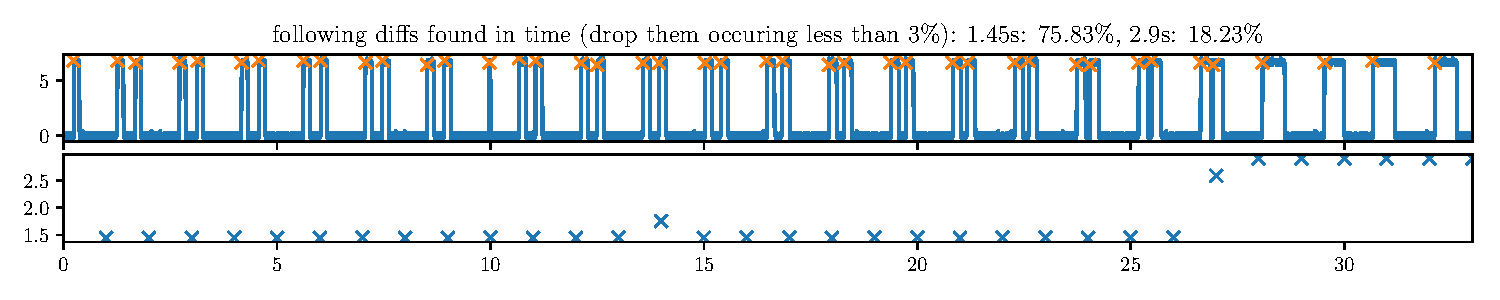
\includegraphics[width=\textwidth]{figures/AufhaengungohneGummi.pdf}
    \caption{Aufhängung ohne fixierende Gummibänder}\label{fig:AufhaengungohneGummi}
\end{figure}
\begin{figure}[htbp]
    \centering
    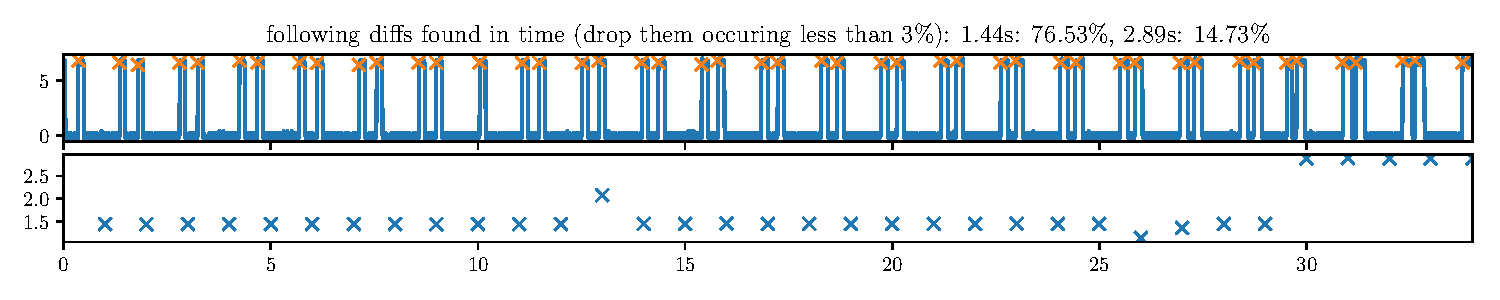
\includegraphics[width=\textwidth]{figures/AufhaengungmitGummi.pdf}
    \caption{Aufhängung mit Halterung}\label{fig:AufhaengungmitGummi}
\end{figure}
\begin{figure}[htbp]
    \centering
    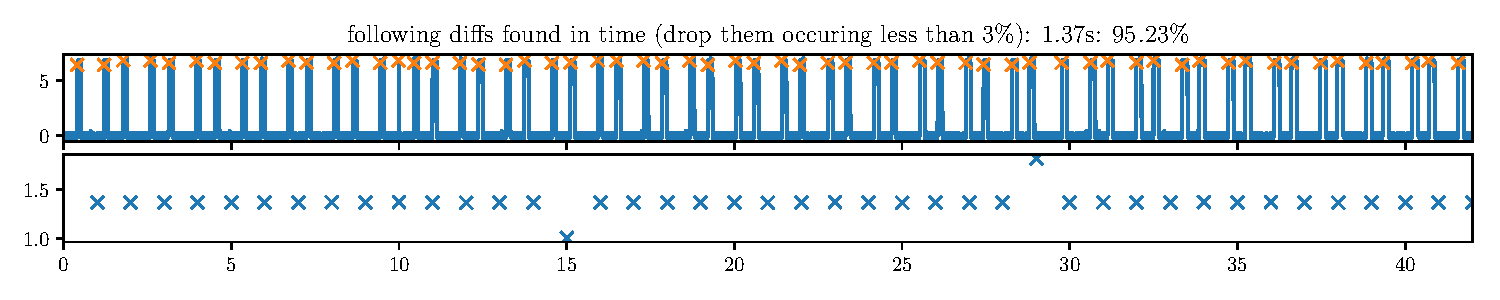
\includegraphics[width=\textwidth]{figures/AufhaengungmitGummiundAuto.pdf}
    \caption{Aufhängung mit befestigtem Auto}\label{fig:AufhaengungmitGummiundAuto}
\end{figure}

\newpage
\section{Radius}
    \begin{table}[tb]
        \caption{Gefahrene Durchmesser und Geschwindigkeiten}
        \label{tab:radius_table1}
        \centering
        \begin{tabular}{|l|l|l|}
        Motorinput & gemittelter Kreisdurchmesser & gemittelte Geschwindigkeit \\ \hline
        300        & 1.2923                       & 0.304                      \\
        500        & 1.2822                       & 0.494                      \\
        1000       & 1.2625                       & 1.181                      \\
        1500       & 1.2755                       & 1.181                      \\
        2000       & 1.2793                       & 1.345                      \\
        2500       & 1.2837                       & 1.498                      \\
        3000       & 1.2941                       & 1.518
        \end{tabular}
    \end{table}
\begin{wraptable}{r}{0.3\textwidth}
    % \begin{table}[tb]
        \caption{Beschleunigende Kreisfahrt (Motorinput 500 - 2600)}
        \label{tab:beschleunigende_kreisfahrt}
        \centering
        \begin{tabular}{|l|}
        Durchmesser in $m$ \\\hline
        1.2856                 \\
        1.2711                 \\
        1.2632                 \\
        1.2492                 \\
        1.2572                 \\
        1.2672                 \\
        1.2691                 \\
        1.2750                 \\
        1.2741                 \\
        1.2720                 \\
        1.2789                 \\
        1.2828                 \\
        1.2817                 \\
        1.2858                 \\
        1.2974                 \\
        1.2965
        \end{tabular}
    \end{wraptable}
    Bei der konstanten Kreisfahrt haben wir sieben Versuchsreihen mit sieben verschiedenen Geschwindigkeiten mittels einer Kamera aufgenommen.
    Die digitalen Werte zur Motoransteuerung sind 300, 500, 1000, 1500, 2000, 2500 und 3000.
    Für jede Geschwindigkeit haben wir mehrer Runden mit konstantem Lenkeinschlag von 25 Grad aufgenommen, um anhand der Aufnahmen die Durchmesser der gefahrenen Kreise zu messen.
    Zu diesem Zweck haben wir eine Referenzstrecke von 60cm in jeder Aufnahme, mit der die gemessenen Längen in den Momentaufnahmen zu den
    realen Längen umgerechnet werden können. Nach Aufnahme der Videos haben wir Momentaufnahmen von Autopositionen alle 180 grad zusammen geschnitten,
    anhand dessen wir die Durchmesser der einzelnen Versuchsreihen messen konnten. Durch dieses Vorgehen konnten wir die gefahrenen Durchmesser und Geschwindigkeiten (Tabelle \ref{tab:radius_table1}) ermitteln können, mit $\text{Umfang} = \pi*\text{Durchmesser}/2$ und $\text{Geschwindigkeit} = \frac{x}{\delta_t}$. $\delta_t$ wurde ebenfalls den Videoaufnahmen entnommen.
    Es ist zu bemerken, dass die Streckenmessung über Momentaufnahmen keine grosse Genauigkeit aufweist und somit ein systematischer Fehler gemacht wird.
    Somit konnten wir auch einen Zusammenhang von Motorinput zu Geschwindigkeit aufstellen (vergleiche Figur \ref{fig:reifenradius}). Hierbei ist ein degressives Verhalten bei höheren Geschw zu erkennen.
    Unter der Annahme eines konstanten Lenkwinkels kann der Eigenlenkgradient $EG$ berechnet werden:
    $EG=(\text{Lenkwinkel}-\text{ackermanwinkel})*R/(v^2)=0.0547\quad (rad*s^2)/m$
    Dabei kann der ackermanwinkel  $l/R = 0.041$ berechnet werden. $l$ ist dabei der Abstand zwischen Vorder- und Hinterreifen.
    (Der Ackermanwinkel wurde für die verschiedenen Radien berechnet und anschliessend gemittelt, da die Abweichungen sehr gering sind.)
    Der positive Eigenlenkgradient deutet auf untersteuerndes Verhalten des Fahrzeugs hin. Dies kann weiter bestätigt werden durch Tabelle \ref{tab:beschleunigende_kreisfahrt}.
    Hier sind die gemessenen Durchmesser bei einer beschleunigenden Kreisfahrt aufgetragen. Da diese bei zunehmender Geschwindigkeit ebenfalls grösser werden, kann auch hier untersteuerndes Verhalten beobachtet werden.
\begin{figure}[hbtp]
        \centering
        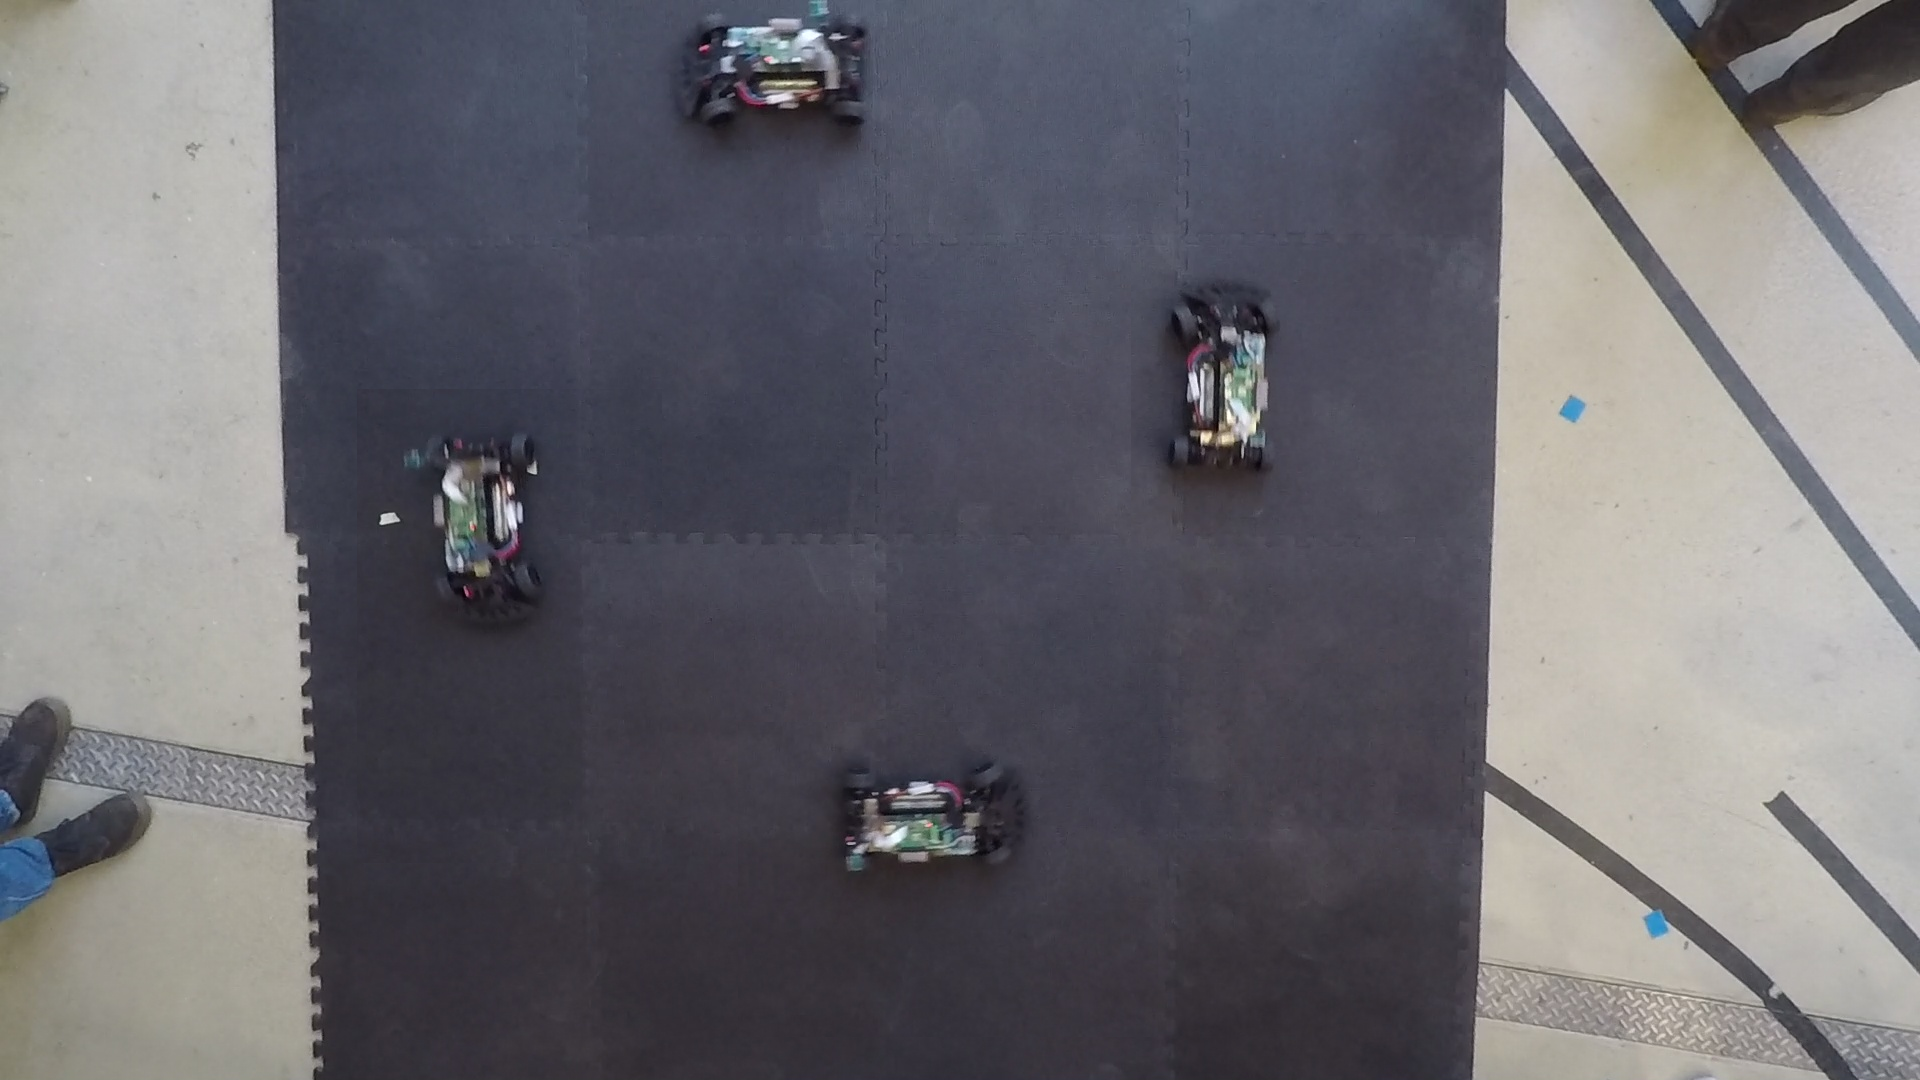
\includegraphics[width=0.7\textwidth]{Dyn_Kreis_5678}
        \caption{Reifenradius}
          % \vspace{-20pt}
        \label{fig:reifenradius}
    \end{figure}


\section{Dynamischer Radius}
    \begin{table}[bthp]
        \caption{Messergebnisse Dynamischer Radius}
        \label{tab:dynamicradius}
        \centering
        \begin{tabular}{|l|l|l|}
        % \hline
        Geschwindigkeit & Umdrehungen & Dynamischer Radius \\ \hline
        1000            & 4,9167      & 3,237 cm           \\
        2000            & 5           & 3,1415 cm          \\
        3000            & 5           & 3,1415 cm
        \end{tabular}
    \end{table}
    Wir haben festgestellt, dass der Durchmesser des Reifens \SI{6,5}{\cm} entspricht.
    Der Radius beläuft sich folglich auf \SI{3,25}{\cm}.
    Bei der Berechnung des dynamischen Radius haben wir die Geschwindigkeiten $1000$, $2000$ und $3000$ verwendet (siehe Tabelle \ref{tab:dynamicradius}).
    Zur Messung haben wir eine Markierung am hinteren linken Reifen angebracht, um die Anzahl der Umdrehungen in einem festen Abstand zu bestimmen (hier: \SI{1}{m}).
    Da der Ausgangsumfang bei \SI{20,42}{\cm} liegt, konnten wir bereits zu Beginn von etwa 5 Umdrehungen ausgehen.
    Hierbei haben wir festgestellt, dass sich der dynamische Radius nur geringfügig von den Ausgangswerten unterscheidet.
    Aufgrund der Messmethode unterliegen diese Ergebnisse allerdings einer gewissen Schwankung.

\section{Motor-Kennlinie}

    \begin{wrapfigure}{r}{0.45\textwidth}
        \centering
        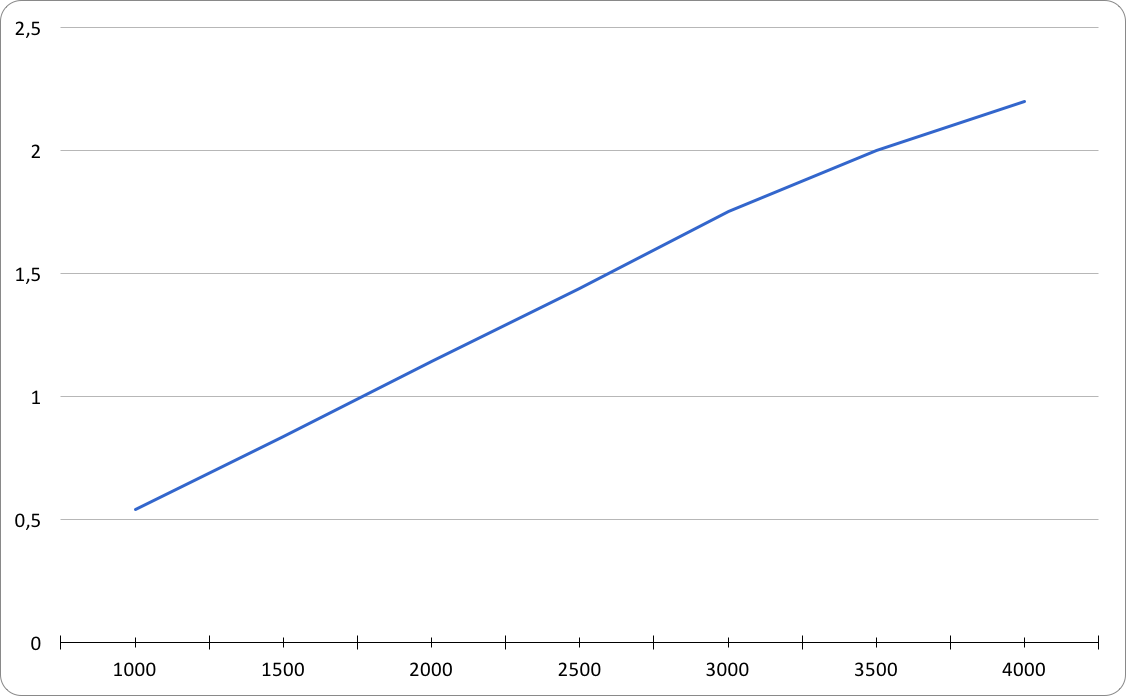
\includegraphics[width=0.4\textwidth]{bild_tim}
        \caption{\SI{1}{\meter\per\second} zu Motorinput}
        \label{fig:m_p_s_zu_motorinput}
    \end{wrapfigure}
    In der Motorkennlinie beobachteten wir lineares Verhalten (vgl. Figur \ref{fig:m_p_s_zu_motorinput}), ausser am Ende der Kennlinie.
    Der Motor arbeitet mit einem Eingang zwischen $0$ und $4095$ Einheiten.
    Beim Aufnehmen der Motorkennlinie mit Python beginnt diese erst bei $1000$ Einheiten;
    erst dort beginnt das Auto, sich zu bewegen.
    Andere Gruppen beobachteten allerdings ein nicht-lineares Verhalten mit fallender Steigung und nahezu logarithmisch verlaufender Kennlinie.
    Zudem liegt die durch uns gemessene Maximalgeschwindigkeit von $4000$ Einheiten unter Vergleichswerten anderer Teams.
    Die Problematik ist uns bewusst und könnte aus unterschiedlicher Modellierung und der Steuerung der Autos resultieren.
    Vor weiterer Modellierung werden wir diesen Aspekt gemeinsam mit anderen Teams weiter untersuchen.


\section{Teamarbeit} % (fold)
\label{sec:teamarbeit}
Dadurch, dass alle Aufgaben von unserem Team gemeinsam gelöst wurden, gab es keine direkte Aufteilung der einzelnen Aufgaben. Wir haben Ideen in Teamarbeit entwickelt und gemeinsam vorangetrieben.
% section teamarbeit (end)


\end{document}
